\pdfminorversion=7
\documentclass[10pt]{article}
\usepackage[margin=0.85in]{geometry}
\usepackage[T1]{fontenc}
\usepackage[utf8]{inputenc}
\usepackage{lmodern}
\usepackage{amsmath,amssymb,amsthm}
\usepackage{booktabs}
\usepackage{tabularx}
\usepackage{enumitem}
\usepackage{xcolor}
\usepackage{listings}
\usepackage{graphicx}
\usepackage{tikz}
\definecolor{bpgreen}{HTML}{1CAC78}
\definecolor{bpdef}{HTML}{B0ECA3}
\definecolor{bpblue}{HTML}{1F5FD6}
\usetikzlibrary{arrows.meta,positioning,shapes.geometric}
\usepackage[colorlinks=true,linkcolor=blue!50!black,citecolor=blue!50!black,urlcolor=blue!50!black]{hyperref}

\graphicspath{{./}{report/}}

\setlist{itemsep=1.5pt,topsep=3pt}
\emergencystretch=3em
\let\origus\_
\renewcommand{\_}{\origus\allowbreak}

\newtheorem{theorem}{Theorem}
\newcommand{\CP}{\mathbb{CP}^1}
\newcommand{\C}{\mathbb{C}}
\newcommand{\R}{\mathbb{R}}
\newcommand{\Z}{\mathbb{Z}}
\newcommand{\N}{\mathbb{N}}
\newcommand{\eps}{\varepsilon}
\newcommand{\code}[1]{\texttt{#1}}

% ---- Auto-populated Repository & Audit Metrics ----
\newcommand{\LeanToolchain}{leanprover/lean4:v4.35.0}
\newcommand{\NModules}{6}
\newcommand{\NLines}{1{,}971}
\newcommand{\NTotalNodes}{21}
\newcommand{\NProvedNodes}{15}
\newcommand{\NDefNodes}{6}
\newcommand{\NLeanDecls}{109}
\newcommand{\NSorryAx}{0}

\lstdefinelanguage{lean}{
  morekeywords={theorem,lemma,def,structure,class,where,by,fun,let,have,exact,obtain,refine,import,namespace,end,variable,open,Nonempty,Fintype},
  sensitive=true, morecomment=[l]{--}, morecomment=[s]{/-}{-/}, morestring=[b]"}
\lstset{language=lean,basicstyle=\ttfamily\scriptsize,keywordstyle=\bfseries\color{blue!50!black},
  commentstyle=\itshape\color{gray},columns=fullflexible,keepspaces=true,frame=single,framerule=0.3pt,
  xleftmargin=4pt,xrightmargin=4pt,breaklines=true,
  literate={→}{{$\to$}}1 {∀}{{$\forall$}}1 {∃}{{$\exists$}}1 {¬}{{$\neg$}}1 {≤}{{$\le$}}1 {≥}{{$\ge$}}1
           {≠}{{$\neq$}}1 {ℕ}{{$\mathbb{N}$}}1 {ℝ}{{$\mathbb{R}$}}1 {ℤ}{{$\mathbb{Z}$}}1
           {ℂ}{{$\mathbb{C}$}}1 {⟨}{{$\langle$}}1 {⟩}{{$\rangle$}}1 {⌊}{{$\lfloor$}}1
           {⌋}{{$\rfloor$}}1 {σ}{{$\sigma$}}1 {ε}{{$\varepsilon$}}1 {ϕ}{{$\phi$}}1
           {κ}{{$\kappa$}}1 {∧}{{$\wedge$}}1 {∘}{{$\circ$}}1 {₁}{{$_1$}}1 {₂}{{$_2$}}1
           {₃}{{$_3$}}1 {₀}{{$_0$}}1 {·}{{$\cdot$}}1 {•}{{$\bullet$}}1 {∨}{{$\vee$}}1
           {⊤}{{$\top$}}1 {<}{{$<$}}1 {>}{{$>$}}1 {‖}{{$\|$}}1 {∈}{{$\in$}}1
           {∂}{{$\partial$}}1 {∫}{{$\int$}}1 {ₗ}{{$_l$}}1 {ᵐ}{{$^m$}}1 {⁻¹}{{$^{-1}$}}1 {ᶜ}{{${}^c$}}1}

\title{\vspace{-1.8em}\textbf{Machine-Checked Formalization of Entropy-Degree Rigidity\\for Non-Collapsed RCD(K, N) Spaces in Lean~4}}
\author{Pablo Su\'arez-Serrato}
\date{November 2026\vspace{-1.0em}}

\begin{document}
\maketitle

\begin{abstract}
\noindent
We present the executive audit and architectural summary of \code{rcd-entropy-degree-rigidity} (Lean~4
package \code{RCDEntropyDegree}), a standalone machine-checked formalization of P.~Su\'arez-Serrato,
\emph{``Entropy-degree rigidity for non-collapsed $\mathsf{RCD}$ spaces''} (2026) in Lean~4
(\code{\LeanToolchain}), built atop the Besson--Courtois--Gallot rank-one determinant engine
\code{BCG} (\code{formalized-barycenter-methods}). Across \NModules{} library modules
(\NLines{} lines of Lean code), \NTotalNodes{} blueprint nodes, and \NLeanDecls{} tracked blueprint
declarations, the entire formalization compiles with \textbf{\NSorryAx{} \code{sorryAx}} and depends
exclusively on Lean's three standard axioms (\code{propext}, \code{Classical.choice}, \code{Quot.sound}).
All \NTotalNodes{} nodes of the \code{leanblueprint} dependency graph are green (\NProvedNodes{} proved
theorem nodes in dark green \code{\#1CAC78} and \NDefNodes{} definition nodes in green \code{\#B0ECA3}).
\end{abstract}

\section{Executive Audit Verdict and Verification Gate}

The formalization of the non-collapsed $\mathsf{RCD}(K, N)$ entropy-degree inequality, its Alexandrov
specialization, and its equality-case isometric rigidity has passed an automated, end-to-end kernel and
blueprint audit executed via \code{verify\_blueprint.py audit}. No custom \code{axiom}, \code{sorry},
\code{admit}, \code{unsafe}, or \code{implemented\_by} occurs anywhere in the repository.

\begin{table}[!ht]
\centering\footnotesize
\renewcommand{\arraystretch}{1.12}
\begin{tabularx}{\textwidth}{@{}>{\bfseries}l l X r@{}}
\toprule
Audit Gate Component & Tool / Target & Verification Scope & Result \\
\midrule
Full Library Compilation & \code{lake build} & \NModules{} library modules (\NLines{} LOC, \code{\LeanToolchain}) & \textbf{Pass} (0 errors) \\
Axiom \& Soundness Census & \code{\#print axioms} & All \NLeanDecls{} declarations in \code{blueprint/lean\_decls} & \textbf{\NSorryAx{} \code{sorryAx}} \\
Foundational Axiom Closure & Kernel inspection & Standard axioms only: \code{\{propext, choice, Quot.sound\}} & \textbf{0 custom axioms} \\
Blueprint Dependency Graph & \code{leanblueprint web} & \NTotalNodes{} total nodes (\code{blueprint/dep\_graph.dot}) & \textbf{100\% Green} (\NProvedNodes{}+\NDefNodes{}) \\
Print \& Report Typesetting & \code{pdflatex} / \code{plasTeX} & \code{blueprint/print/print.pdf} \& report generation & \textbf{0 \code{plasTeX} errors} \\
\bottomrule
\end{tabularx}
\caption{Summary of the automated verification gate (\code{verify\_blueprint.py audit}).}
\label{tab:audit}
\end{table}

\section{Mathematical Achievements: The Master Theorem}

The repository formalizes the extension of the Besson--Courtois--Gallot barycenter method \cite{BCG1995}
from smooth manifolds to closed orientable non-collapsed $\mathsf{RCD}(K, N)$ metric-measure spaces
\cite{DPG2018} and closed orientable $N$-dimensional Alexandrov spaces without boundary
\cite{SuarezSerrato2026}.

\begin{theorem}[$\mathsf{RCD}(K, N)$ and Alexandrov Entropy-Degree Rigidity]\label{thm:rcd_main}
Let $(X, \mathsf{d}, \mathcal{H}^N)$ be a closed orientable non-collapsed $\mathsf{RCD}(K, N)$ space with
CMMP orientation current $T \in \mathbf{I}_N(X)$ \cite{CMMP}, and let $f : X \to Y$ be a continuous map to
a closed oriented negatively curved locally symmetric $N$-manifold $Y$ with universal-cover volume
entropy $h(\widetilde{Y}) > 0$.
\begin{enumerate}[label=\textbf{(\arabic*)}]
\item \emph{(Entropy-Degree Inequality)} Writing $h(\overline{X})$ for the volume entropy of the
universal cover $\overline{X}$ of $X$,
\[
|\deg(f)|\, h(\widetilde{Y})^N \, \mathcal{H}^N(Y) \;\le\; h(\overline{X})^N \, \mathcal{H}^N(X).
\]
When $X$ is a closed orientable $N$-dimensional Alexandrov space of curvature $\ge \kappa$ without
boundary, the specialization $K = (N - 1)\kappa$ yields the Alexandrov entropy-degree theorem; when
Mitsuishi's comparison homomorphism relates $\deg(f) = m_X \cdot \mathrm{ind}_H(f)$, the same bound
holds with $\mathrm{ind}_H(f)$ in place of $|\deg(f)|$.
\item \emph{(Equality-Case Rigidity)} Suppose $k = |\deg(f)| = [\pi_1(Y) : f_*\pi_1(X)] \ge 1$ and
equality holds: $h(\overline{X})^N \mathcal{H}^N(X) = k\, h(\widetilde{Y})^N \mathcal{H}^N(Y)$.
For the degree-$k$ Riemannian cover $p : \widehat{Y} \to Y$ associated to $f_*\pi_1(X)$, lift
$\hat{f} : X \to \widehat{Y}$, rescaling factor $c = h(\overline{X}) / h(\widetilde{Y}) > 0$, and
$1$-Lipschitz limit map $\hat{F}_\infty : X \to \widehat{Y}$ homotopic to $\hat{f}$, we have
$|\deg(\hat{f})| = 1$, $c^N \mathcal{H}^N(X) = \mathcal{H}^N(\widehat{Y})$,
$\mathrm{Jac}_x \hat{F}_\infty = 1$ $\mathcal{H}^N_c$-a.e., $\hat{F}_\infty$ is surjective, and
by Lipschitz-volume rigidity \cite{LiWang}, $\hat{F}_\infty : (X, c\,\mathsf{d}_X) \to \widehat{Y}$ is a
global metric isometry while $p \circ \hat{F}_\infty : X \to Y$ is a $k$-sheeted Riemannian covering.
\end{enumerate}
\end{theorem}

\paragraph{Lean~4 Formulations.}
\begin{enumerate}\sloppy
\item \textbf{Inequality \& Rank-One Dispatch (\code{RCDEntropyDegree/RCD/EntropyDegreeRigidity.lean}).}
\code{rcd\_entropy\_degree\_inequality} proves Part~(1) directly from the pushforward mass-Jacobian
bound and the scale-wise BCG entropy inequality (\code{BCG.bcg\_volume\_entropy\_inequality});
\code{rcd\_rankOne\_entropy\_degree\_theorem} dispatches the tangent-space Busemann Hessian implicit
equation to \code{BCG.rankOne\_bcg\_main\_theorem} across all rank-one targets $\mathbb{K}\mathbf{H}^m$;
\code{alexandrov\_entropy\_degree\_inequality} and \code{rcd\_homological\_index\_entropy\_inequality}
specialize Part~(1) to Alexandrov spaces and Mitsuishi's homological index.
\item \textbf{Equality-Case Rigidity (\code{ae\_jacobian\_eq\_one\_of\_normalized\_equality},
\code{rcd\_entropy\_degree\_equality\_rigidity}).} Combines the finite-cover degree reduction
(\code{finite\_cover\_entropy\_degree\_reduction}), homothetic normalization
(\code{homothetic\_normalization}), the a.e.\ mass-Jacobian sandwich, degree surjectivity
(\code{surjective\_of\_degree\_ne\_zero}), and Lipschitz-volume rigidity into a single theorem.
\end{enumerate}

\begin{lstlisting}[caption={Master entropy-degree inequality and equality rigidity signatures in \code{RCDEntropyDegree.RCD}.}]
theorem rcd_entropy_degree_inequality
    (C : CMMPOrientationCurrent X K N CurrentX) [IsFiniteMeasure C.hausdorffMeasure]
    (FY : FundamentalManifoldCurrent Y CurrentY) {h_Xbar h_Ytilde : ℝ} (hh_Ytilde : 0 < h_Ytilde)
    {deg_f : ℤ} (F_s : ℝ → X → Y) (D_s : ∀ s : ℝ, s > h_Xbar → LipschitzDegreePushforward C FY (F_s s))
    (Jac_s : ℝ → X → ℝ) (h_deg_homotopy : ∀ (s : ℝ) (hs : s > h_Xbar), (D_s s hs).lipschitzDegree = deg_f)
    (h_mass_push : ∀ (s : ℝ) (hs : s > h_Xbar),
      FY.totalMass (D_s s hs).pushforwardCurrent ≤ ∫ x, Jac_s s x ∂C.hausdorffMeasure)
    (hJac_int : ∀ s > h_Xbar, Integrable (Jac_s s) C.hausdorffMeasure)
    (hJac_bound : ∀ s > h_Xbar, ∀ᵐ x ∂C.hausdorffMeasure, Jac_s s x ≤ (s / h_Ytilde) ^ N) :
    |(deg_f : ℝ)| * h_Ytilde ^ N * FY.manifoldVolume ≤ h_Xbar ^ N * C.totalVolume

theorem rcd_entropy_degree_equality_rigidity [CompactSpace X] [T2Space Yhat]
    (C_rescaled : CMMPOrientationCurrent X K N CurrentX) [IsFiniteMeasure C_rescaled.hausdorffMeasure]
    (FYhat : FundamentalManifoldCurrent Yhat CurrentYhat)
    {k deg_fhat h_Xbar h_Ytilde vol_X vol_Y : ℝ} (hk_pos : 0 < k) (hh_Xbar : 0 < h_Xbar) (hh_Ytilde : 0 < h_Ytilde)
    (hdeg_mult : k = k * deg_fhat) (hvol_cover : FYhat.manifoldVolume = k * vol_Y)
    (heq : entropyVolumeProduct N h_Xbar vol_X = k * entropyVolumeProduct N h_Ytilde vol_Y)
    (hvol_rescaled : C_rescaled.totalVolume = (h_Xbar / h_Ytilde) ^ N * vol_X)
    {Fhat_inf : X → Yhat} (hFhat_cont : Continuous Fhat_inf)
    (D_inf : LipschitzDegreePushforward C_rescaled FYhat Fhat_inf) (Jac_inf : X → ℝ)
    (hD_deg_ne : D_inf.lipschitzDegree ≠ 0) (hD_deg_abs : |(D_inf.lipschitzDegree : ℝ)| = deg_fhat)
    (h_open_pos : ∀ U : Set Yhat, IsOpen U → U.Nonempty → 0 < (FYhat.volumeMeasure U).toReal)
    (h_supp : (FYhat.massMeasure (D_inf.lipschitzDegree • FYhat.fundamentalClass) (Set.range Fhat_inf)ᶜ).toReal = 0)
    (h_mass_push : FYhat.totalMass D_inf.pushforwardCurrent ≤ ∫ x, Jac_inf x ∂C_rescaled.hausdorffMeasure)
    (hJac_int : Integrable Jac_inf C_rescaled.hausdorffMeasure)
    (hJac_le_one : ∀ᵐ x ∂C_rescaled.hausdorffMeasure, Jac_inf x ≤ 1)
    (h_lip_vol_rigidity : Function.Surjective Fhat_inf → C_rescaled.totalVolume = FYhat.manifoldVolume →
      (∀ᵐ x ∂C_rescaled.hausdorffMeasure, Jac_inf x = 1) →
      ∀ x₁ x₂ : X, dist (Fhat_inf x₁) (Fhat_inf x₂) = (h_Xbar / h_Ytilde) * dist x₁ x₂) :
    let c := h_Xbar / h_Ytilde; 0 < c ∧ deg_fhat = 1 ∧ c⁻¹ * h_Xbar = h_Ytilde ∧
    c ^ N * vol_X = FYhat.manifoldVolume ∧ C_rescaled.totalVolume = FYhat.manifoldVolume ∧
    (∀ᵐ x ∂C_rescaled.hausdorffMeasure, Jac_inf x = 1) ∧ Function.Surjective Fhat_inf ∧
    (∀ x₁ x₂ : X, dist (Fhat_inf x₁) (Fhat_inf x₂) = c * dist x₁ x₂)
\end{lstlisting}

\section{Architectural Synthesis: Unconditional Proofs vs.\ Interfaces}

\begin{table}[!ht]
\centering\footnotesize
\renewcommand{\arraystretch}{1.12}
\begin{tabularx}{\textwidth}{@{}>{\bfseries}l c X@{}}
\toprule
Architectural Chapter & Nodes & Principal Proved Achievements (\code{\#1CAC78}) \\
\midrule
Ch.\ 1: Volume Entropy \& Scaling & 4 & Basepoint independence, hyperbolic Bishop--Gromov growth density bound, isometric/equivariant exponential weights, homothetic \& finite-cover reduction (\code{MetricMeasure/VolumeEntropy.lean}). \\
Ch.\ 2: Sturm $\mathrm{CAT}(0)$ Barycenter & 4 & Renormalized $d^2$-functional continuity, linear growth, midpoint deficit \& Sturm variance uniqueness, $\pi_1$-equivariant natural maps, geodesic homotopy descent (\code{MetricMeasure/SturmBarycenter.lean}). \\
Ch.\ 3: $\mathsf{RCD}(K,N)$ \& CMMP Currents & 4 & Codimension-two singular stratification $\mathcal{S}(X)\subseteq\mathcal{S}^{N-2}$, Alexandrov specialization, and CMMP orientation current mass \& singular-nullity laws (\code{RCD/StructureAndCurrents.lean}). \\
Ch.\ 4: Degree \& Homotopy Invariance & 4 & Regular value openness \& full measure ($V_f = Y \setminus f(\mathcal{S}(X))$), Lipschitz pushforward degree identity, Wenger homotopy invariance, surjectivity, and homological index (\code{RCD/DegreeTheory.lean}). \\
Ch.\ 5: Jacobians \& Rigidity & 5 & Metric Jacobian, pushforward mass-Jacobian bound (Lemma~3.3), pointwise entropy-Jacobian bound via \code{BCG}, Theorem~1.1 Parts~1--2 (\code{RCD/EntropyDegreeRigidity.lean}). \\
\bottomrule
\end{tabularx}
\caption{Breakdown of the \NTotalNodes{} blueprint nodes (\NProvedNodes{} proved theorem nodes, \NDefNodes{} definition nodes).}
\label{tab:layers}
\end{table}

\paragraph{1. Unconditionally Proved Pillars.}
All metric-measure volume entropy bounds, Bishop--Gromov hyperbolic growth estimates, normalized
exponential weight $\pi_1$-equivariance, Sturm's $\mathrm{CAT}(0)$ $d^2$-barycenter existence/uniqueness
(via the $\mathrm{CAT}(0)$ variance inequality \code{sturm\_variance\_inequality}), geodesic homotopy
descent to quotients, regular-value openness/full-measure lemmas, algebraic pushforward degree identities,
the finite-cover \& homothetic rescaling reductions, the mass-Jacobian sandwich
(\code{ae\_jacobian\_eq\_one\_of\_normalized\_equality}), and the upstream rank-one Busemann Hessian
determinant bound dispatched via \code{BCG} are proved unconditionally from Mathlib first principles.

\paragraph{2. Typed Metric-Measure \& Geometric-Measure Interfaces.}
Deep metric-geometric foundational theorems not yet available in Mathlib~4 are encapsulated inside
explicit hypothesis structures without introducing any \code{axiom} declarations:
\code{NonCollapsedRCDStructure} / \code{AlexandrovSpaceWithoutBoundary} (De~Philippis--Gigli regularity
and codimension-two stratification \cite{DPG2018}), \code{CMMPOrientationCurrent} (the CMMP integral
$N$-current on closed orientable $\mathsf{RCD}(K,N)$ spaces \cite{CMMP}),
\code{LipschitzDegreePushforward} (Sormani--Wenger / Kirchheim area and homotopy constancy
\cite{Wenger2011,CDNPSW2025}), and the explicit Lipschitz-volume rigidity hypothesis
\code{h\_lip\_vol\_rigidity} (Li--Wang / Connell--et~al.\ \cite{LiWang,CDNPSW2025}) in Theorem~1.1 Part~2.

\section{Modular Dependency Architecture and Verification Pipeline}

\begin{figure}[!ht]
\centering
\resizebox{\textwidth}{!}{%
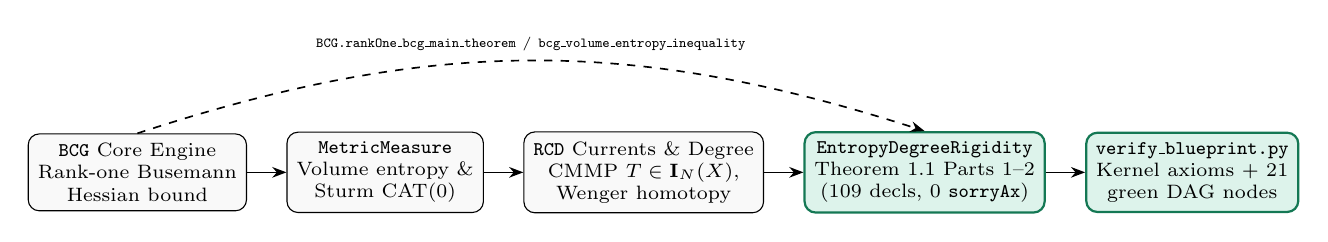
\begin{tikzpicture}[node distance=4.5mm and 5.0mm, every node/.style={font=\scriptsize},
  box/.style={draw,rounded corners,align=center,inner sep=3.5pt,minimum height=7.5mm,fill=gray!5},
  gate/.style={draw,rounded corners,align=center,inner sep=3.5pt,minimum height=7.5mm,fill=bpgreen!15,
               draw=bpgreen!70!black,thick},
  arr/.style={-{Stealth[length=1.8mm]},semithick}]
\node[box] (bcg) {\code{BCG} Core Engine\\Rank-one Busemann\\Hessian bound};
\node[box,right=of bcg] (mm) {\code{MetricMeasure}\\Volume entropy \&\\Sturm $\mathrm{CAT}(0)$};
\node[box,right=of mm] (rcd) {\code{RCD} Currents \& Degree\\CMMP $T \in \mathbf{I}_N(X)$,\\Wenger homotopy};
\node[gate,right=of rcd] (thm) {\code{EntropyDegreeRigidity}\\Theorem 1.1 Parts 1--2\\(\NLeanDecls{} decls, \NSorryAx{} \code{sorryAx})};
\node[gate,right=of thm] (ver) {\code{verify\_blueprint.py}\\Kernel axioms + \NTotalNodes{}\\green DAG nodes};
\draw[arr] (bcg)--(mm);
\draw[arr] (mm)--(rcd);
\draw[arr] (rcd)--(thm);
\draw[arr] (thm)--(ver);
\draw[arr,dashed] (bcg.north) to[bend left=18] node[above,font=\tiny]{\code{BCG.rankOne\_bcg\_main\_theorem} / \code{bcg\_volume\_entropy\_inequality}} (thm.north);
\end{tikzpicture}%
}
\caption{Package architecture linking \code{BCG} (\code{formalized-barycenter-methods}) to \code{RCDEntropyDegree} and automated verification.}
\label{fig:pipeline}
\end{figure}

Downstream applications of the Alexandrov entropy-degree theorem (Su\'arez-Serrato,
\code{arXiv:2606.30403}) consume \code{RCDEntropyDegree} in the companion repository
\code{alexandrov-entropy-degree-applications}.

\begin{thebibliography}{99}\footnotesize\sloppy
\setlength{\itemsep}{1pt}
\bibitem{BCG1995} G.~Besson, G.~Courtois, S.~Gallot, Entropies et rigidit\'es des espaces localement
  sym\'etriques de courbure strictement n\'egative, \emph{Geom.\ Funct.\ Anal.} \textbf{5} (1995), 731--799.
\bibitem{Sturm2003} K.-T.~Sturm, Probability measures on metric spaces of nonpositive curvature,
  \emph{Contemp.\ Math.} \textbf{338} (2003), 357--390.
\bibitem{Wenger2011} S.~Wenger, Flat convergence for integral currents in metric spaces,
  \emph{Calc.\ Var.\ Partial Differential Equations} \textbf{40} (2011), 423--449.
\bibitem{DPG2018} G.~De~Philippis, N.~Gigli, Non-collapsed spaces with Ricci curvature bounded from
  below, \emph{J.\ \'Ec.\ polytech.\ Math.} \textbf{5} (2018), 613--650.
\bibitem{CMMP} N.~Cavallucci, S.~Marti, A.~Mondino, R.~Perales, Integral currents and orientation in
  non-collapsed $\mathsf{RCD}(K, N)$ spaces.
\bibitem{CDNPSW2025} C.~Connell, X.~Dai, J.~N\'u\~nez-Zimbr\'on, R.~Perales, P.~Su\'arez-Serrato,
  G.~Wei, Lipschitz-volume rigidity and stability bounds on $\mathsf{RCD}(K,N)$ spaces.
\bibitem{LiWang} Z.~Li, R.~Wang, Volume rigidity for Lipschitz maps on $\mathsf{RCD}(K,N)$ spaces.
\bibitem{SuarezSerrato2026} P.~Su\'arez-Serrato, Entropy-degree rigidity for non-collapsed $\mathsf{RCD}$
  spaces (2026).
\end{thebibliography}

\newpage
\appendix
\section{Blueprint Dependency Graph}\label{app:graph}

\begin{center}
\vspace{0.5em}
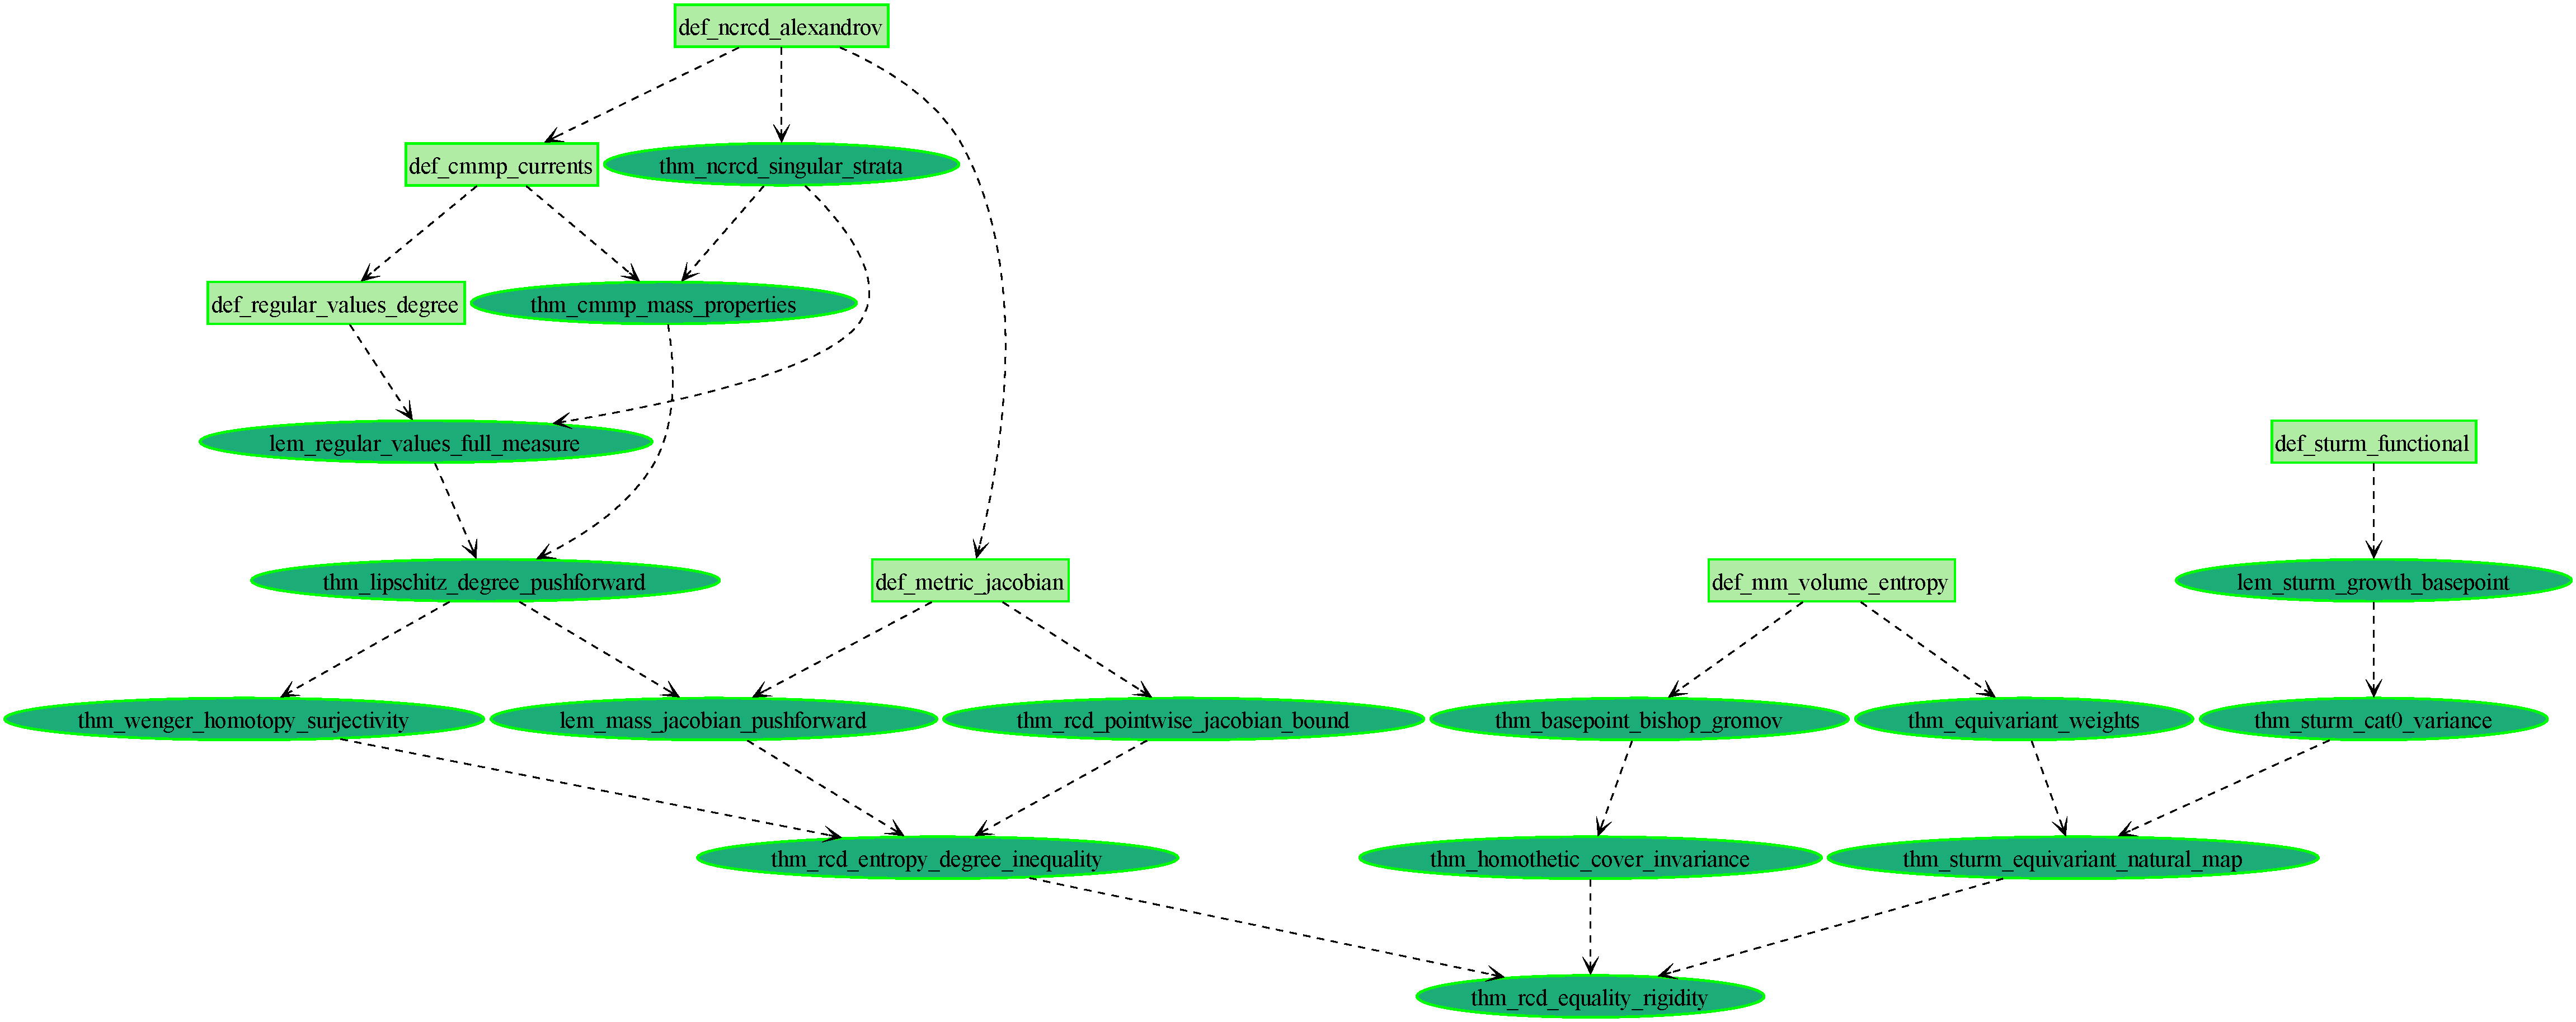
\includegraphics[width=\linewidth,height=0.80\textheight,keepaspectratio]{blueprint_dep_graph.pdf}
\end{center}
\vspace{0.5em}
\noindent\footnotesize\sloppy
\textbf{Figure A.1: Complete \code{leanblueprint} Dependency Graph (Portrait View).}
Generated from \code{blueprint/src/content.tex} via \code{build\_dep\_graph.py}
(interactive HTML version at \code{blueprint/web/dep\_graph\_document.html}).
Arrows point from each foundational definition or lemma to the downstream theorems that depend on it.
\textbf{Node shapes and colors:}
\textbf{Rectangles (\NDefNodes{} nodes, green \code{\#B0ECA3}):} Formalized mathematical definitions.
\textbf{Ellipses (\NProvedNodes{} nodes, dark green \code{\#1CAC78}):} Fully machine-checked theorems,
lemmas, and certificates compiling with \code{0 sorryAx} and standard Lean~4 axioms across
the entire dependency closure.
\textbf{Unproved nodes:} $0$ light green (\code{\#9CEC8B}), $0$ light blue (\code{\#A3D6FF}).\par

\end{document}
